\subsection{Requirement Interpretation and IP Selection}
The first stage determines the reusable system components required by the target application. Directly mapping natural-language descriptions to concrete IP instances is unreliable because user terminology, IP metadata, and hardware interfaces are expressed at different abstraction levels. SoCPilot therefore separates requirement interpretation from IP retrieval. As shown in Figure \ref{fig:soc-spec}, the LLM first converts the user description into a structured SoC specification and then uses this specification to query a hierarchical library of verified IPs.



The structured specification records three types of information: (1) the required system functions, such as sensing, communication, and application processing; (2) quantitative constraints, including latency, throughput, power, area, and memory capacity; and (3) integration attributes, such as data types, protocols, and external interfaces. Missing or ambiguous fields trigger an interactive clarification step. This representation decomposes a high-level application scenario into explicit IP categories and target specifications, providing a stable interface between user intent and the implementation flow.

\begin{table*}[htb]
\centering
\begin{threeparttable}
  \caption{Requirement-to-IP Taxonomy for SoC Customization}
  \label{tab:req_taxonomy}
  \begin{tabularx}{0.8\linewidth}{cllX}
    \toprule
    \textbf{Tier\tnote{a}} & \textbf{Category} & \textbf{Tag} & \textbf{Description / Examples} \\
    \midrule
    \multirow{1}{*}{T0} 
      & Application Domain       & \texttt{domain} & AI inference, sensor hub, audio DSP, ISPs, etc. \\
    \midrule
    \multirow{4}{*}{T1}
      & Compute                  & \texttt{cpu}, \texttt{dsp}, \texttt{ai} & RISC-V, Arm cores, DSPs, AI accelerators\\
      & Memory and Cache         & \texttt{mem}     & DDR/LPDDR, SRAM, cache hierarchy and coherency, scratchpad \\
      & Interconnect             & \texttt{noc}, \texttt{axi}, \texttt{pcie} & Mesh NoC, AXI buses, PCIe root complex \\
      & I/O Interfaces           & \texttt{io}      & USB, SPI, I2C, CAN, MIPI CSI/DSI, GPIO \\
    \midrule
    \multirow{4}{*}{T2}
      & Power and Energy         & \texttt{power}   & Power budget, DVFS, retention memory \\
      & Security and Safety      & \texttt{sec}     & AES engine, secure boot, ASIL level \\
      & Reliability / Lifetime   & \texttt{rel}     & ECC, watchdog, over-temperature protection \\
      & Thermal and Packaging    & \texttt{pkg}     & Thermal budget, packaging constraints \\
    \midrule
    \multirow{1}{*}{T3}
      & Integration Constraints  & \texttt{pkg}     & I/O count, physical interface compatibility (e.g., PHYs, pads) \\
    \bottomrule
  \end{tabularx}
  
  % 表格下方的注释区域
  \begin{tablenotes}
    \footnotesize
    \item[a] T0 identifies the application domain; T1 describes primary hardware components; T2 captures cross-layer constraints; and T3 records implementation and integration constraints.
  \end{tablenotes}
  
\end{threeparttable}
\end{table*}

Table~\ref{tab:req_taxonomy} summarizes the taxonomy used to organize both requirements and IP metadata. Each library entry contains a functional description, supported configurations, interface protocols, resource and performance characterization, verification status, and known dependencies. SoCPilot first retrieves semantically similar verified designs from a case library. If no case provides a compatible configuration, the LLM decomposes the structured specification into IP queries, retrieves candidates from the hierarchical IP library, and filters them using hard constraints such as protocol compatibility, capacity, and resource limits. The remaining candidates are ranked by their match to the requested performance targets.

The output of this stage is a machine-readable SoC manifest that records the selected processor, memory hierarchy, interconnect, I/O components, and their initial configurations. Application-specific compute kernels are not assumed to exist in the reusable IP library; instead, their accelerator implementations are determined by the profiling and hardware/software partitioning stage described next. This separation prevents the requirement interpreter from prematurely deciding which application functions should be implemented in hardware.
\begin{figure*}[htp]
    \centering
    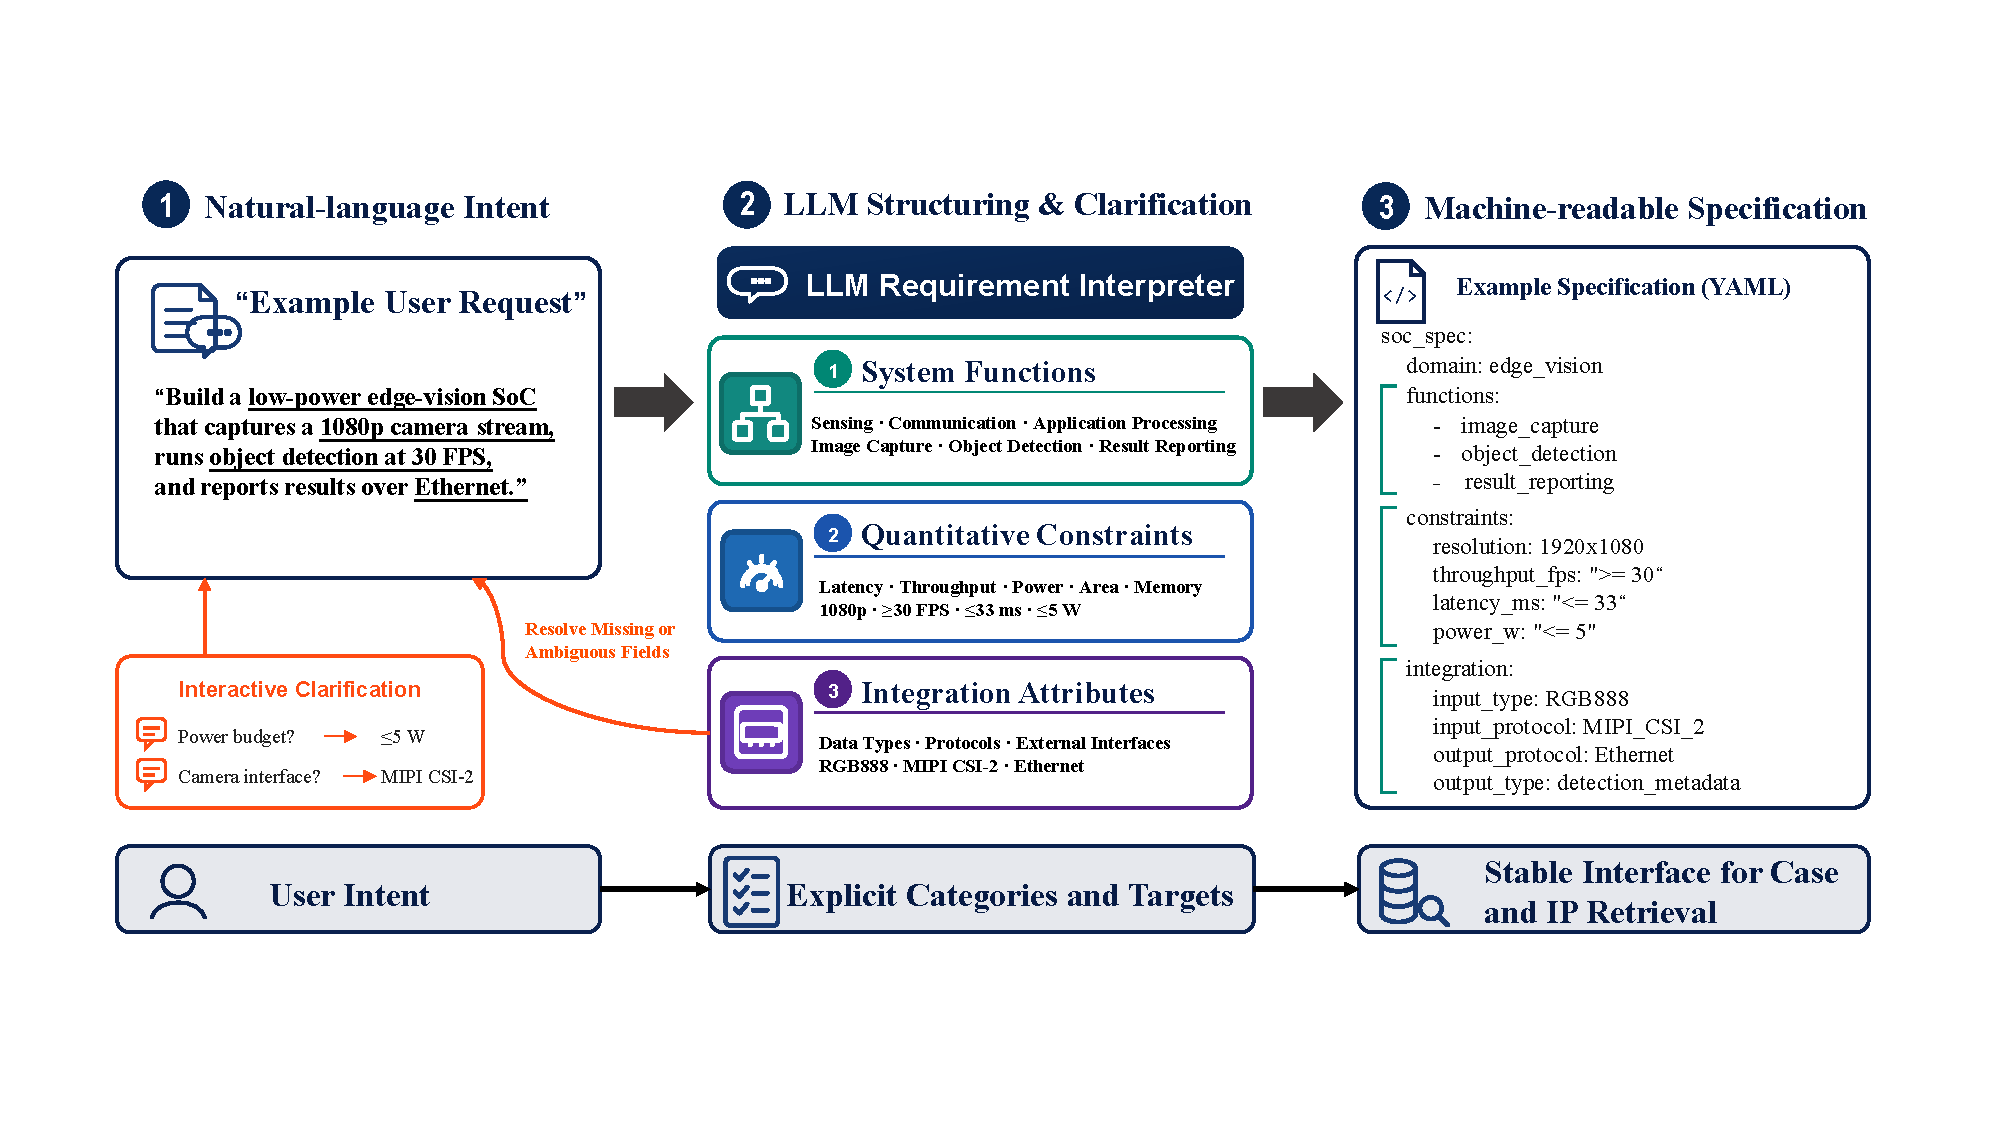
\includegraphics[width=0.95\textwidth]{pic/soc-spec.pdf} 
    \caption{Structured SoC specification generation. The LLM translates natural-language requirements into system functions, quantitative constraints, and integration attributes, while resolving missing or ambiguous fields through interactive clarification. The example illustrates the resulting machine-readable specification used for subsequent case and IP retrieval.}
\label{fig:soc-spec}
    \vspace{-1em}
\end{figure*}
